\documentclass[a4paper,12pt,twoside]{memoir}
\usepackage{longtable}
\usepackage{btp}    % Use the trainermanual package option (i.e. \usepackage[trainermanual]{btp}) to generate the Trainer's version of the manual
%\usepackage[
%  noinfo,
%  cam,
%  cross,                % crosses as marks
%  a4,
%  width=6.25in,         % the width of the galley
%  height=9.25in,        % the height of the galley
%  center                % actual page is centered on the galley
%]{crop}
% Set some Workshop specific info
\setWorkshopTitle{Implementing Scalable Bioinformatic Workflows in Snakemake and Nextflow}
\setWorkshopVenue{Across Australia}
\setWorkshopDate{Aug/Sep 2019}
\setWorkshopAuthor{
Nathan S. Watson-Haigh\\
Radosław Suchecki\\
}


\lstset{
 literate={~} {$\sim$}{1} % set tilde as a literal (no process)
}

\begin{document}

%
% Workshop Title Page
%
\workshoptitlepage

%
% CC-BY
%
\input{licences/licence.tex}
\clearpage

\setcounter{tocdepth}{2}
\tableofcontents

\chapter{Workshop Information}
\clearpage

%
% Trainers Page
%
\section{The Trainers}

\newlength{\trainerIconWidth}
\setlength{\trainerIconWidth}{2.0cm}

\begin{center}
\begin{longtable}{>{\centering\arraybackslash} m{1.1\trainerIconWidth} m{1\textwidth}}

  % Use the following block of commended LaTeX as a template for each trainer taking part in the workshop

  % ---- START TEMPLATE ---- %
  %\includegraphics[width=\trainerIconWidth]{photos/generic.jpg} &
  %  \textbf{Dr. Jane Bloggs}\newline
  %  Research Fellow in Bioinformatics\newline
  %  The Blogg Institute, Somewhere\newline
  %  \mailto{jane.bloggs@example.com}\\
  % ----- END TEMPLATE ----- %

  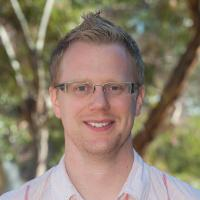
\includegraphics[width=\trainerIconWidth]{photos/Watson-Haigh.jpeg} &
    \textbf{Dr. Nathan S. Watson-Haigh}\newline
    Senior Bioinformatician\newline
    Bioinformatics Hub, University of Adelaide\newline
    \mailto{nathan.watson-haigh@adelaide.edu.au}\\

  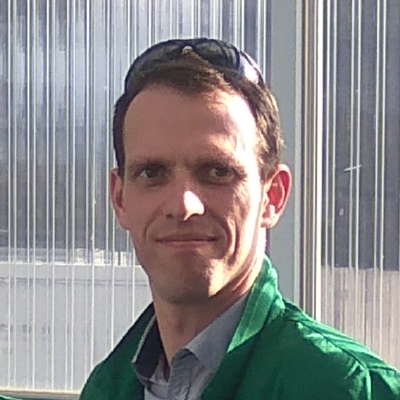
\includegraphics[width=\trainerIconWidth]{photos/Suchecki.png} &
    \textbf{Dr. Rados{\l}aw Suchecki}\newline
    Research Scientist\newline
    Crop Bioinformatics and Data Science, CSIRO\newline
    \mailto{rad.suchecki@csiro.au}\\
  
\end{longtable}
\end{center}



%
% Workshop Preamble
%
%
% Start: General Information describing the workshop and the structure of the handouts
%
\newpage

\section{Providing Feedback}
While we endeavour to deliver a workshop with quality content and documentation in a venue
conducive to an exciting, well run hands-on workshop with a bunch of knowledgeable and likable
trainers, we know there are things we could do better.

Whilst we want to know what didn't quite hit the mark for you, what would be most helpful and least
depressing, would be for you to provide ways to improve the workshop. i.e. constructive feedback.
After all, if we knew something wasn't going to work, we wouldn't have done it or put it into the
workshop in the first place!

Clearly, we also want to know what we did well! This gives us that ``feel good'' factor which will
see us through those long days and nights in the lead up to such hands-on workshops!

With that in mind, we'll provide a some high tech mechanism through which you
can provide anonymous feedback during the workshop:
\begin{enumerate}
%  \item A sheet of paper, from a flip-chart, sporting a ``happy'' face and a ``not so happy'' face.
%  Armed with a stack of colourful post-it notes, your mission is to see how many comments you can
%  stick on the ``happy'' side!
  
  \item Some empty ruled pages at the back of this handout. Use them for your own personal notes or
  for writing specific comments/feedback about the workshop as it progresses.
  
%  \item An online post-workshop evaluation survey. We'll ask you to complete this before you leave.
%  If you've used the blank pages at the back of this handout to make feedback notes, you'll be able
%  to provide more specific and helpful feedback with the least amount of brain-drain!
\end{enumerate}

\section{Document Structure}
We have provided you with an electronic copy of the workshop's hands-on tutorial documents.
We have done this for two reasons: 1) you will have something to take away with you at the 
end of the workshop, and 2) you can save time (mis)typing commands on the command line by using
copy-and-paste.

\emph{We advise you to use Acrobat Reader to view the PDF. This is because it properly supports some
features we have implemented to ensure that copy-and-paste of commands works as expected. This
includes the appropriate copy-and-paste of special characters like tilde and hyphens as well as
skipping line numbers for easy copy-and-past of whole code blocks.}

\begin{warning}
While you could fly through the hands-on sessions doing copy-and-paste, you will learn more if you
use the time saved from not having to type all those commands, to understand what each command is
doing!
\end{warning}

The commands to enter at a terminal look something like this:
\begin{lstlisting}
snakemake --profile profiles/slurm --use-singularity --printshellcmds all 
\end{lstlisting}  

The following icons are used in the margin, throughout the documentation to help you navigate around
the document more easily:

% TODO limit the use of some icons throughout as some are clearly overused and confuse the eye
\hspace*{.2cm}\vcent{\includegraphics[height=1cm]{icons/info.png}} Important\\
\hspace*{.2cm}\vcent{\includegraphics[height=1cm]{icons/notes.png}} For reference\\
\hspace*{.2cm}\vcent{\includegraphics[height=1cm]{icons/steps.png}} Follow these steps\\
\hspace*{.2cm}\vcent{\includegraphics[height=1cm]{icons/questions.png}} Questions to answer\\
\hspace*{.2cm}\vcent{\includegraphics[height=1cm]{icons/warning.png}} Warning - STOP and read\\
\hspace*{.2cm}\vcent{\includegraphics[height=1cm]{icons/bonus1.png}} Bonus exercise for fast learners\\
\hspace*{.2cm}\vcent{\includegraphics[height=1cm]{icons/bonus2.png}} Advanced exercise for super-fast learners\\

%========================
\section{Provided Compute Infrastructure}
%========================

For the purposes of this training, we are providing you with access to a virtual cluster running on top of
AWS. The specification of this cluster is as follows:

\begin{description}[style=multiline,labelindent=0cm,align=left,leftmargin=0.5cm]
  \item[Head Node]\hfill\\
    \texttt{m5d.4xlarge} (16 vCPU, 64G RAM and 2x300 SSD)
  \item[Compute Nodes]\hfill\\
    \texttt{t2.medium}, min: 30 max: 50
  \item[Shared Storage]\hfill\\
    \texttt{1000G}
\end{description}

%========================
\subsection{Connecting to the Cluster}
%========================

\begin{steps}
First up, lets connect to the head node of the HPC cluster using \texttt{ssh}.

\emph{See your local facilitator for connection details. You will have one user account per person.}

Upon connecting, feel free to use \texttt{screen} or \texttt{tmux} if you are familiar with either of those tools.

\end{steps}

%========================
\subsection{Monitoring Slurm Jobs}
%========================

\begin{note}

You can monitor all jobs in the slurm squeue, or just your own job(s) using the slurm command \texttt{squeue}:

\begin{lstlisting}
# All jobs in the queue
squeue

# Just your own jobs
squeue --user ${USER}
\end{lstlisting}

For convienience we have provided you with the \texttt{sq} function which produces nicer output than the default \texttt{squeue}:

\begin{lstlisting}
# All jobs in the queue
sq

# Just your own jobs
sq --user ${USER}
\end{lstlisting}

\end{note}


%
% Start of modules
% Switch chapter styling to module
%
\chapterstyle{module}


%
% End of modules
% Switch back to normal workshop chapter styling
%
\chapterstyle{workshop}

\chapter{Space for Personal Notes or Feedback}
\clearpage

%
% Some empty ruled comments pages
%
\myruledpage{0cm}{1cm}
\myruledpage{0cm}{1cm}
\myruledpage{0cm}{1cm}
\myruledpage{0cm}{1cm}

\end{document}
